\documentclass[10pt]{report}

\usepackage[a4paper]{geometry}

\usepackage{amsmath,amsfonts,amsthm}

\usepackage{graphicx}

\usepackage{booktabs}

\usepackage{siunitx}

\usepackage{url}

\usepackage{caption}
\usepackage{subcaption}
\usepackage{multirow}

\usepackage{hyperref}
	\hypersetup{colorlinks=false,pdfborder=0 0 0}

\usepackage{cleveref}
	\crefname{equation}{equation}{equations}
	\crefname{figure}{figure}{figures}	
	\crefname{table}{table}{tables}


\usepackage[utf8]{inputenc}

\usepackage[english]{babel}
	
\usepackage[backend=bibtex, style=authoryear, sorting=nty]{biblatex}
\bibliography{refs/references.bib}

\usepackage{listings}

\usepackage{float}

\usepackage{pdflscape}

\usepackage{bm}

\usepackage[toc,page]{appendix}

\newcommand{\thickhat}[1]{\mathbf{\hat{\text{$#1$}}}}
\theoremstyle{plain}
\newtheorem{thm}{Theorem}
\theoremstyle{definition}
\newtheorem{defn}{Definition}




\author{Alexander James Waudby}
\title{Credit Scorecard Modelling}
\date{\today}

\begin{document}

\maketitle

\newgeometry{left=5cm,right=5cm}
\begin{abstract}
The acceptance or rejection of a creditee is a difficult task for the lender. On one hand, every applicant is potential profit but on the other, they all come with varying risks of defaulting and potential loss. The lenders have many tools for maximinzing their profit whilst maintaining a low risk. One such method is credit scorecards and scorecard modelling. By using previous applicants data we can develop a score of potential new applicants and their risk of being unable to repay their loan. In this project I will first introduce some of the methods used in scorecard modelling and then apply these to a real world data set, producing several scorecards and comparing their performance. We found that a logistic regression was capable of developing a suitable model for this data set. Finally I will demonstate the scorecards ability to be applied to other fields of study by reapplying the methods done on the credit score data onto a data set of patients with covid-19 and producing a health risk scorecard on the outcome of a patient.
\end{abstract}
\restoregeometry

\tableofcontents

\listoffigures

\chapter{Credit Scoring}

\section{Introduction}
Credit scoring is a method used by financial institution globally to assess whether a customer should be taken on. This can be for a variety of services such as credit cards, loans, mortgages, etc. It's development originated from the need of risk vs rewards. Lenders needed a way of determining if a potential customer would be able to pay back their credit and as such not costing the lender money by taking on creditees which end up being unable to repay the debt. A credit score is usually just a number indicating your quality as a creditee. The scale of the score can vary on which lender is providing the score but usual ones are 0-999 or 0-500 with the lower the score the less likely you would be offered the service. \\

Although used globally, there is no widely accepted "perfect" model or method. All companies assess their customers differently, a customer could be rejected from one lender and be accepted by another based on what they would define as an acceptable client. Even within companies the models and methods can change due to new circumstances and the changing financial climet. What previously could of been a strong predictor of a bad client could now be insignifcant. A recent example of this is the technology development of mobile phones. Previously, if a client did not have access home phone this could be an indicator of a possible bad client. Now, with the development and wide public access to mobile phones, access to a home phone has become mostly irrelevant with most of the public having no use for them anymore. Changes such as this and others require lenders to be constantly evaluating how they assess customers to prevent the rejection of good clients and the accepting of bad ones.

\section{Modelling}
Credit score modelling is often discrete based with the most common being a logistic regression with the response variable being either a good $(y=0)$ or bad customer $(y=1)$. Predictors can be a variety of variable such as personal characteristics, age, gender or economic status e.g. car owner, home owner/rentor etc, to financial characteristics like amont of current debt and repayment statuses. One thing to note, certain personal characteristics are off limit to company due to discrimination laws. Predictors such as race, may be shown to have some use in scoring but cannot be used as the model would become discriminatory.

\section{WOE and IV}
Weight of evidence (WOE) is a popular method used in score card modelling, often used because the variables used in credit scoring can have a large amount of categories which cause impractiallities when converting these to dummy variables. WOE is an alternative to that, rather than create a large amount of dummy variables, the method produces a numerical value (weight of evidence) for each category which is prdouced by (\ref{WOE}). with $f()$ being the distribution of category $X$ for goods and bads. These value then replace their respective categorical value when modelling the scorecard.

\begin{equation}\label{WOE}
WOE = \ln \frac{f(X=x|y=0)}{f(X=x|y=1)}
\end{equation}

IV, the information value. Is a measure of the weight of evidence for categories $IV \geq 0$. A value of 0 indicates the variable has no predictive power i.e. no valueable information in the variable. IV is calculated by (\ref{IV}). A guideline produced by Bailey\cite{bailey2004credit} is below for evaluating the IV values.

\begin{equation}\label{IV}
\textup{IV} = \sum (\% \textup{ of Bad} - \% \textup{ of Good}) \cdot \textup{WOE}
\end{equation}

\begin{figure}[H]
	\centering
	\begin{tabular}{l l l l}
	IV	&Recommendation \\
	\hline
	Less than 0.03			&Poor Predictor \\
	From 0.03 to less than 0.10	&Weak Predictor \\
	From 0.10 to less than 0.30	&Average Predictor \\
	From 0.30 to less than 0.50	&Strong Predictor \\
	Over 0.50				&Very Strong Predictor \\
	\end{tabular}
	\caption{Information Value Table \label{Table1}}\cite{bailey2004credit}
\end{figure}

\section{Performance Evaulation}

\subsection{ROC and AUC}
ROC, Receiver Operating Characteristic. Was a method of analysis developed during World War II under "Signal Detection Theory". It was originally used for radar operators and their ability to determine if a blip on screen was an enemy or just noise, hence the name Receiver Operating Characteristics.\cite{tape2000using} Since then, the method has been applied into a variety of fields for visuallising the accuary of classification models. \\

Understanding the ROC Curve is relatively simple, the plot is the false positive rate against true positive rate for different cutoff points. The true positive rate is seen as the sensitivity and the false positive being (1 - specificity) An example figure can be found below, the higher the curve, the more accurate the model can be seen as, with the neutral line going 45 degrees through the plot can be seen as the model being the same as a 50/50 guess on the outcome. In some cases these curves can overlap and cause some ambiguity on which curve is overall the best so the measure used to remove this amiguity is the AUC, Area under the curve (\ref{AUC}). A higher AUC inidicates a stronger disciminatory power with 0.5 being none and 1 being a "perfect model". As such the model with a higher AUC can be considered "a better model". Generally, an $AUC > 0.8$ is considerd good.

\begin{equation}\label{AUC}
A = \int_{c}^{} F_1(c){F_0}'(c) dc
\end{equation}

A more common representation of the AUC is the gini coefficient (\ref{GINI}). A linear transformation of the AUC to allow the measure to have a preferred 0 to 1 scale rather than 0.5 to 1.

\begin{equation}\label{GINI}
gini = (2 \cdot AUC) - 1
\end{equation}

\subsection{K-S Statistic}

The K-S Statistic (Kolmogorov-Smirnov Statistic) is a measurement of the scorecards ability to seperate the goods from bads. The K-S Statistic is the maximum distance between the cumulative distributions of both the goods and bads, or alterntively, if $F_{g}(x)$ is the cumulative distribution of goods and bads is $F_{b}(x)$ where $x$ is the score then the KS Statistic is (\ref{KS})

\begin{equation}\label{KS}
KS = max(F_{g}(x) - F_{b}(x))
\end{equation}

The statistic can be expressed visually by plotting the cumlative distributions as seen below. An issue of this measurement is that it only provides the score at which the scordcard seperates the goods and bads the most. The cutoff score for the card might not necessarily be this score and a higher K-S score does not imply the scorecard is a better fit. 

\subsection{Divergence}

Divergence is a measurement of the distributions of goods and bads. The idea is that the scorecard on average will assign a lower score to bads than goods i.e. $\mu_{b} < \mu_{g}$. Divergence is a way to assess this performance. 

\section{Cut-off}
A scorecard in simple terms is just a method producing a score for each individual. To put the scorecard into use the difference between the scores needs to be classified this is done by a cut-off score. This score is a point on the scorecard which would seperate accepted applicants from rejected. A simple cut-off method would be to have a single score, any applicants above the score are accepted and anyone below the score is rejected. The benefit of a simple method is the ability to quickly process applicants and move desired applicants onto the next stage faster. The issue with the single cutoff comes with the applicants that are close to the cutoff, having a strict cut-off can cause a company to take on bad applicants or reject good applicants where futher investigation would prove the applicant more likely to be the opposite. \\

An alternative to this would be a two score cut-off. This would be done by having two scores like $ \textup{Rejected } < S_{1} < \textup{ Refer } < S_{2} < \textup{ Accepted}$. Any score above $S_{2}$ is automatically accepted and any below $S_{1}$ is rejected. Scores which the land in between and moved to a referral stage where a lender can further look into the applicants case by case to decide the outcome. This comes with added benefit of removing the issue of applicants close to the single cutoff. The idea is that with the lenders insight, more good applicants will be accepted and more bads rejected compared to the single cutoff, thus possibly reducing the bad rate of accepted applicants. \\

The cut-off scores can be determined by varying factors which can change depending on the companies interest. Four of these are specified by Bailey \cite{bailey2004credit}. Acceptance rate, the percentage of all applicants accepted by the cut-off. Overall bad rate, the percentage of all accepted applicants that end up being bads. Marginal bad rate, the percentage of accepted applicancts that are bad close to the cut-off score. Profitability, the possible profit from goods minus the loss from bads. Depending on the situation of the business and its goals would determine the importance of each factor with overal bad rate being the usual priority.



%\begin{figure}[H]
%	\centering
%	\includegraphics[scale=0.50]{figs/White_Pop}
%	\caption{\% Of White Alone population in Boston Metropolitan \label{W_Pop}}\cite{DataCommon}
%\end{figure}
%
%\begin{figure}[H]
%	\centering
%	\includegraphics[scale=0.50]{figs/Black_Pop}
%	\caption{\% Of Black or African American population in Boston Metropolitan \label{B_Pop}}\cite{DataCommon}
%\end{figure}
%
%\begin{figure}[H]
%	\centering
%	\includegraphics[scale=0.50]{figs/Asian_Pop}
%	\caption{\% Of Asian alone population in Boston Metropolitan \label{A_Pop}}\cite{DataCommon}
%\end{figure}

%The state of Metro Boston's Economy is considered one of the stronger economies when compared to state, national averages and globally. In a report done by Brookings Insitute  in 2014 of 300 of the world's largest metropolitan economies, Boston ranked in at 24th in the world for GDP with \$ 360,110 million and 4th for GDP per capita with \$ 76,204.\cite{GMM} The economy of Boston is heavily influenced by its' financial, business and technological services along with the city having strong educational and medical sectors. Home to leading medical schools Tufts University and Harvard University and also Massachusetts Institute of Technology, International students come from come from all over the world to study at the world class universities in Boston. The affect of having prestigious universities in a city can have a large impact on the economy of the city. The high skilled work force they produce has attracted the knowledge-based industries on which Boston's economy is now heavily based. Examples of these are the high technology, biotechnology and financial service. Boston boasts a very strong educational sector and produces numerous skilled professionals. Along with these, Boston is also a popular tourist destination with both domestic and international visitors. In 2014 visitors spent \$12.2 billion.\\
%
%The costs of living in Boston according to Numbeo's index can be considered to be at a high standard.\cite{NUM} The index can be seen as the cost of living in an area relative to what it is in New York. In 2014 Boston was ranked 121 of 473 globally and 14 of 94 in North America with a cost of living index of 92.94 (New York being 100.00). \\
%
% The city's median household income is one of the higher for the Nations cities with average value of \$58,263. Although the city still contains the racial disparities for incomes seen across the country. The median household income is comparatively very low when you reach the inner part of the city with some areas having an average income less than \$ 40,000. This also follows along with the racial income gaps, with the average median income for an African American household being at \$40,128 and \$80,515 for a White household.\cite{CityData}
 
%\begin{figure}[H]
%	\centering
%	\includegraphics[scale=0.50]{figs/Med_Inc}
%	\caption{Median household income \label{Med_Inc}}\cite{DataCommon}
%\end{figure} 
%
%\begin{figure}[H]
%	\centering
%	\begin{tabular}{l l l l}
%	Date	&US		&Massachusets	&Boston \\
%	\hline
%	2015	&\$55,775	&\$70,628	&\$78,800 \\
%	2014	&\$53,719	&\$69,240	&\$75,754 \\
%	2013	&\$53,167	&\$67,939	&\$74,186 \\
%	2012	&\$53,031	&\$67,451	&\$74,057 \\
%	2011	&\$53,223	&\$66,246	&\$73,197 \\
%	2010	&\$54,405	&\$67,479	&\$73,945 \\
%	2009	&\$55,478	&\$70,789	&\$76,592 \\
%	2008	&\$57,276	&\$71,997	&\$78,558 \\
%	2007	&\$58,003	&\$71,291	&\$77,895 \\
%	2006	&\$56,957	&\$70,490	&\$75,405 \\
%	2005	&\$56,122	&\$69,402	&\$75,329 \\
%	\end{tabular}
%	\caption{Historical Inflation Adjusted Median Household Income for Boston \label{Table1}}\cite{HouseholdIncome}
%\end{figure}

\chapter{Literature Review}\label{chapter:2}

\section{Cut-off}

A scorecard, in simple terms, is just a sum of points producing a total score for each individual. To put the scorecard into use the difference between the scores needs to be classified. This is done by the cut-off score. The cut-off score is a point on the scorecard which would seperate accepted applicants from the rejected. A simple cut-off method would be to have a single score, any applicants above this score are accepted and anyone below the score is rejected. The benefit of a simple method is the ability to quickly process applicants and move desired applicants onto the next stage faster. The issue with the single cut-off comes with the applicants that are close to the cut-off, having a strict cut-off can cause a company to take on bad applicants or reject good applicants where futher investigation would prove the applicant to more likely be the opposite. \\

An alternative to this would be the two score cut-off. This would be done by having two scores like $ \textup{Rejected } < S_{1} < \textup{ Refer } < S_{2} < \textup{ Accepted}$. Any score above $S_{2}$ is automatically accepted and any below $S_{1}$ is rejected. Scores which then land in between are then moved to a referral stage where a lender can further look into the applicants case by case to decide the outcome. This comes with added benefit of removing the issue of applicants being close to the single cut-off. The idea is that with the lenders insight, more good applicants will be accepted and more bads rejected compared to the single cut-off, thus possibly reducing the bad rate [\ref{sec:glossary}] of accepted applicants. \\

The cut-off scores can be determined by varying factors which can change depending on the companies interest. Four of these are specified by \parencite{bailey2004credit}. Acceptance rate, the percentage of all applicants accepted by the cut-off. Overall bad rate, the percentage of all accepted applicants that end up being bads. Marginal bad rate, the percentage of accepted applicancts that are bad that are also close to the cut-off score. Profitability, the possible profit from goods minus the loss from bads. Depending on the situation of the business and its goals would determine the importance of each factor with overal bad rate being the usual priority.

\pagebreak

\section{Weight of evidence and Information value}  \label{sec:woe_and_iv}

Weight of evidence, WOE. Is a popular method used for data preperation in scorecard modelling. Often used because, the variables can either have a large amount of categories, which would require creation of many dummy variables. Or, the numerical variables do not follow a linear relationship with the goods and bads, creating difficulties for the logistic regression when assigning a coefficient. An example of this issue can be seen later in Section (\ref{sec:variables}) and the variable CLNO, the variable will also be used as an example here. WOE is a solution to these problems, rather than creating many dummy variables, the method produces a numerical value (weight of evidence) for each category/bin. The binning method used to create the bins for WOE is detailed in Section (\ref{chimerge}). WOE is produced by Equation (\ref{WOE}). 

\begin{equation}\label{WOE}
WOE = \ln \frac{f(X=x|y=1)}{f(X=x|y=0)}
\end{equation}

where $f()$ is the distribution of category $X$ for either goods $(y=0)$ or bads $(y=1)$. \\

For the example we have the variable CLNO which has been binned into the boundaries in Table (\ref{table:woe_example_table}). To calculate the WOE for the bin $[10, 20)$ we do the following. 

\begin{equation}\label{WOE_Example}
\begin{aligned}
f(X=x|y=1) =& \dfrac{293}{876} = 0.3345 \\
f(X=x|y=0) =& \dfrac{1589}{4094} = 0.3881 \\
WOE =& \ln \dfrac{0.3345}{0.3881} \\
WOE =& -0.15
\end{aligned}
\end{equation}

where 293 is the number of bads in the bin, 876 is the total number of bads in the data, 1589 is the number of goods in the bin and 4094 is the total number of goods in the data. \\

\begin{table}[H]
\centering
		\begin{tabular}{lllrrrrrrrr}
		\toprule
		variable & bin &  good &  bad  &       woe  \\
		\midrule
		     CLNO &  [-inf, 10.0)  &   323 &  156  &  0.81  \\
		     &  [10.0, 20.0) &  1589 &  293  & -0.15  \\
		     &  [20.0, 21.0)&   221 &   76  &  0.47  \\
		     &  [21.0, 24.0) &   505 &   95  & -0.13 \\
		     &  [24.0, 26.0)&   369 &   34  & -0.84 \\
		     &   [26.0, inf)  &  1087 &  222  & -0.05  \\
		\midrule
		     &		        & 4094 & 876 & \\
		\bottomrule
		\end{tabular}
		\caption{CLNO Binning \label{table:woe_example_table}}
\end{table}

The values produced by this would then replace the value of each observation which lies in the respective category/bin before using whichever modelling method used to develop the scorecard.  \\

The information value, IV. Is a measure of the weight of evidence $IV \geq 0$. A value of 0 indicates the variable has no predictive power i.e. no valuable information in the variable. IV can be calculated by Equation (\ref{IV}). A guideline produced by \parencite{bailey2004credit} is below for evaluating the IV values in Table (\ref{table:IV}).

\begin{equation}\label{IV}
\textup{IV} = \sum (\% \textup{ of Bad} - \% \textup{ of Good}) \cdot \textup{WOE}
\end{equation}

\begin{table}[H]
	\centering
	\begin{tabular}{l l l l}
	IV	&Recommendation \\
	\hline
	Less than 0.03			&Poor Predictor \\
	From 0.03 to less than 0.10	&Weak Predictor \\
	From 0.10 to less than 0.30	&Average Predictor \\
	From 0.30 to less than 0.50	&Strong Predictor \\
	Over 0.50				&Very Strong Predictor \\
	\end{tabular}
	\caption{Information Value Table \label{table:IV}}\parencite{bailey2004credit}
\end{table}

Taking the example of CLNO again with Table (\ref{table:woe_example_table}). We can calculate the IV by doing the following.

\begin{equation}\label{IV_Example}
\begin{aligned}
IV =& \sum_{i}^{N} (\dfrac{B_{i}}{B} - \dfrac{G_{i}}{G}) \cdot \textup{$WOE_{i}$} \\
IV =& 0.15
\end{aligned}
\end{equation}

where $N$ is the total number of bins, $i$ is the ith bin, $B_{i}$ and $G_{i}$ are the number of bads and goods in bin i, B and G are the total number of goods and bads and $WOE_{i}$  is the WOE value of bin i.

\section{Performance Evaulation} \label{sec:perf_eval}

\subsection*{ROC and AUC}
Receiver Operating Characteristic, ROC. Was a method of analysis developed during World War II under ``Signal Detection Theory". It was originally used for radar operators and their ability to determine if a blip on screen was an enemy or just noise, hence the name Receiver Operating Characteristics \parencite{tape2000using}. Since then, the method has been applied into a variety of fields for visuallising the accuary of classification models. \\

Understanding the ROC Curve is relatively simple, the plot is the false positive rate against true positive rate for different cut-off points. The true positive rate is seen as the sensitivity and the false positive being (1 - specificity). An example can be seen in Figure (\ref{roc_example}), the higher the curve, the more accurate the model can be seen as, with the neutral line going 45 degrees through the plot being seen as the model being the same as a 50/50 guess on the outcome. In some cases these curves can overlap and cause some ambiguity on which curve is overall the best so the measure used to remove this amiguity is the Area under curve, AUC (\ref{AUC}). A higher AUC inidicates a stronger disciminatory power with 0.5 being none and 1 being a ``perfect model". As such the model with a higher AUC can be considered ``a better model". Generally, an $AUC > 0.8$ is considerd good.

\begin{equation}\label{AUC}
A = \int_{c}^{} F_1(c){F_0}'(c) dc
\end{equation}

A more common representation of the AUC is the gini coefficient (\ref{GINI}). A linear transformation of the AUC to allow the measure to have a preferred 0 to 1 scale rather than 0.5 to 1.

\begin{equation}\label{GINI}
gini = (2 \cdot AUC) - 1
\end{equation}

\begin{figure}[!ht]
	\centering
	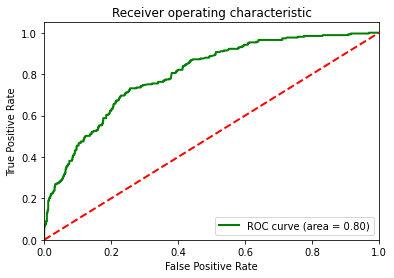
\includegraphics[scale=1.00]{figs/roc_example.png}
	\caption{ROC Example \label{roc_example}}
\end{figure}

\subsection*{K-S Statistic}

The K-S Statistic (Kolmogorov-Smirnov Statistic) is a measurement of the scorecards ability to seperate the goods from bads. The K-S Statistic is the maximum distance between the cumulative distributions of both the goods and bads. This can be calculate by Equation (\ref{KS}). \\

\begin{equation}\label{KS}
K-S = max(F_{g}(x) - F_{b}(x))
\end{equation}

where $F_{g}(x)$ is the cumulative distribution of goods at score $x$ and $F_{b}(x)$ is the distribution of bads at score $x$. \\

An issue of this measurement is that it only provides the score at which the scorecard seperates the goods and bads the most. The cut-off score for the card might not necessarily be this score and a higher K-S score does not imply the scorecard is a better fit. 

\subsection*{Divergence}

Divergence is a measurement of the distributions of goods and bads created by the scorecard. The idea is that the scorecard on average will assign a lower score to bads than goods i.e. $\mu_{b} < \mu_{g}$. Divergence is a way to assess this performance. Specified by \parencite{bailey2004credit} divergence is calculated by Equation (\ref{eq:divergence})

\begin{equation}\label{eq:divergence}
Divergence = \dfrac{(\mu_g - \mu_b)^2}{\dfrac{1}{2} (\sigma_g^2 + \sigma_b^2)}
\end{equation}

where $\mu$ is the mean and $\sigma^2$ is the variance and g and b are goods and bads respectively

\subsection*{Population Stability Index}

The population stability index, PSI. Is a measure of the distributions of two populations to ensure similarity. Credit score models are developed using historical data and it is important to ensure that the data used to model the scorecard does not differ too much from the data the model will be used to assess. A high PSI can result in investigation as the use of the model could potentially be unsuitable and cause an increase in risk from the company \parencite{yurdakul2018statistical}. Although the data being used is collected in the same time period, PSI can still be used to compare train and test data sets to ensure there isn't a large population shift between the two.\\

Interpretation of the PSI in the industry is not set in stone. The general guideline mentioned by \parencite{bailey2004credit} is that a psi of less than 10\% indicates no shift, 10 to 25\% shows a slight shift and should be investiaged and a PSI greater than 25\% suggests the model should be revaluated on more recent data. PSI can be calculated using the Equation (\ref{eq:psi})\parencite{yurdakul2018statistical}.

\begin{equation}\label{eq:psi}
PSI = \sum_{i=1}^{B} (y_i-y_{b_i}) * ln(\dfrac{y_i}{y_{b_i}})
\end{equation}

where $y_i$ is the proportion of target year credit scores that fall in the ith bin, $y_{b_i}$ is the proportion of base year credit scores than fall in the ith bin and B represents the number of bins.

\section{Data Cleaning Methods} \label{sec:data_cleaning}

Missing data is a problem that comes with any raw dataset that you might come across and there are a variety of methods to handling them. Missing data can be categorised into 3 types, missing completely at random, MCAR. Missing at random, MAR, and missing not at random, MNAR. The most common assumption is that the data is MAR, missing data is not missing because of the value but rather a function from some other observered variable. (e.g. an applicant with category A may not want to disclose the value of the variable. Where as an applicant in category B is more likely to disclose). MCAR is when the probability of missingness is unrelated to the observed variables such as a study participant not returning for a follow-up, etc. MNAR is when the variable is missing due to the value of the variable, for example someone may not want to disclose their income if they consider it to be on the lower end \parencite{buhi2008out}. Determining what category the variable lies in is often impossible in practice as to determine if a variable is MNAR you would need to know what those missing values are to compare with the values not missing which is often not available \parencite{newman2014missing}.\\

For this project we decided to use a mixture of data cleaning methods, regression imputation, single imputation and listwise deletion. Regression imputation is the use of other available data to develop a regression model to predict the missing values. Single imputation is the use of the available data from the variable and impute the same value for each, e.g. the use of mean, median or mode as the value for the remaining. Listwise deletion is the removal of any observation with missing data remaining.

\section{Chimerge Discretization} \label{chimerge}

For the application of the woe methods a python package called scorecardpy will be used to help automate the process by finding the optimal bins for the numerical variables. The package has the two options for optimizing, tree based and chimerge. For this project we will be using the chimerge method and will explain its application here. \\

The chimerge methods uses the $\chi^2$ statistic to bin numerical variables. It can be seen in detail in \parencite{kerber1992chimerge}. The intial step is for the variables to be sorted and then each observation will be split into its own bin. Each bin will then be compared to its adjacent and calculate the $\chi^2$ value, the bin is then merged into the adjcent bin with the lowest $\chi^2$ value. This step is repeated until all pairs have $\chi^2$ values exceeding a threshold. The formula for computing $\chi^2$ can be seen in Equation (\ref{CHI}).

\begin{equation}\label{CHI}
\chi^2 = \sum^{m}_{i=1}\sum^{k}_{j=1} \dfrac{(A_{ij} - E_{ij})^2}{ E_{ij}}
\end{equation}

where, m = 2, the two intervals being compared. k is the number of classes, in our case 2 (Good and Bad). $A_{ij}$ is the number of observations in ith interval and jth class. $E_{ij}$ is the expected frequency of $A_{ij}$ which is calculated by Equation (\ref{AFREQ}).

\begin{equation}\label{AFREQ}
A_{ij} = \dfrac{R_i - C_j}{N}
\end{equation}

where, $R_i$ is the number of observations in ith interval. $C_j$ is the number of observations in jth class and N is the total number of observations.



\chapter{Modelling} \label{cha:chapter-3}

\section{Logistic Regression}

\section{Results}

Data was split into train and test sets with proportions 0.7 and 0.3 respectively. Bad rate was maintained in each data set at 17\%. The woe values from tables  (\ref{woe_1}) \& (\ref{woe_2}) were applied. Once split the train data was passed through a glm model with logit link, for this the statsmodel package was used \cite{statsmodels}. Three models were run and compared  (\ref{glm_out}).  

\begin{figure}
\begin{center}
\begin{tabular}{lclc}
\toprule
\textbf{Dep. Variable:}  &       BAD        & \textbf{  No. Observations:  } &     3522    \\
\textbf{Model:}          &       GLM        & \textbf{  Df Residuals:      } &     3510    \\
\textbf{Model Family:}   &     Binomial     & \textbf{  Df Model:          } &       11    \\
\textbf{Link Function:}  &      logit       & \textbf{  Scale:             } &    1.0000   \\
\textbf{Method:}         &       IRLS       & \textbf{  Log-Likelihood:    } &   -1236.8   \\
\textbf{Date:}           & Sat, 15 Aug 2020 & \textbf{  Deviance:          } &    2473.6   \\
\textbf{Time:}           &     13:16:04     & \textbf{  Pearson chi2:      } &  3.55e+03   \\
\textbf{No. Iterations:} &        6         & \textbf{                     } &             \\
\bottomrule
\end{tabular}
\begin{tabular}{lcccccc}
                      & \textbf{coef} & \textbf{std err} & \textbf{z} & \textbf{P$> |$z$|$} & \textbf{[0.025} & \textbf{0.975]}  \\
\midrule
\textbf{const}        &      -1.6002  &        0.054     &   -29.683  &         0.000        &       -1.706    &       -1.495     \\
\textbf{CLNO\_woe}    &       0.8862  &        0.154     &     5.755  &         0.000        &        0.584    &        1.188     \\
\textbf{REASON\_woe}  &      -0.1580  &        0.455     &    -0.347  &         0.729        &       -1.051    &        0.735     \\
\textbf{VALUE\_woe}   &       0.8818  &        0.159     &     5.558  &         0.000        &        0.571    &        1.193     \\
\textbf{YOJ\_woe}     &       1.1226  &        0.214     &     5.238  &         0.000        &        0.703    &        1.543     \\
\textbf{DELINQ\_woe}  &       1.0389  &        0.072     &    14.443  &         0.000        &        0.898    &        1.180     \\
\textbf{LOAN\_woe}    &       0.7584  &        0.115     &     6.581  &         0.000        &        0.533    &        0.984     \\
\textbf{DEROG\_woe}   &       0.8037  &        0.100     &     8.062  &         0.000        &        0.608    &        0.999     \\
\textbf{CLAGE\_woe}   &       0.8006  &        0.102     &     7.861  &         0.000        &        0.601    &        1.000     \\
\textbf{NINQ\_woe}    &       1.0246  &        0.139     &     7.397  &         0.000        &        0.753    &        1.296     \\
\textbf{JOB\_woe}     &       0.7379  &        0.155     &     4.764  &         0.000        &        0.434    &        1.041     \\
\textbf{MORTDUE\_woe} &       0.0044  &        0.234     &     0.019  &         0.985        &       -0.455    &        0.464     \\
\bottomrule
\end{tabular}
\caption{Generalized Linear Model Regression Results \label{glm_out}}
\end{center}
\end{figure}

\begin{figure}
\begin{center}
\renewcommand{\arraystretch}{1.25}
\begin{tabular}{lccc}
\toprule
Model & AIC & KS & GINI \\
Model 1 (Default) & 2497.64 & 0.4616 & 0.5985 \\
Model 2 (REASON and MORTDUE dropped) & 2493.76 & 0.4584 & 0.5985 \\
Model 3 (Log transformations) & 2504.0873 & 0.4753 & 0.5993 \\
\bottomrule
\end{tabular}
\caption{Performance Evaluation Results On Test \label{perf_eval}}
\end{center}
\end{figure}

\begin{figure}[!ht]
	\centering
	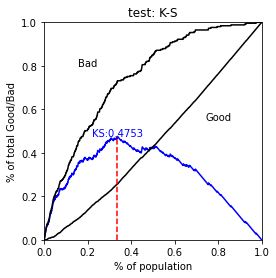
\includegraphics[scale=0.90]{figs/ks_plot.png}
	\caption{KS Plot \label{ks_plot}}
\end{figure}

\begin{figure}[!ht]
	\centering
	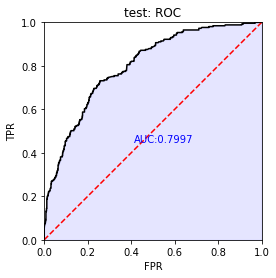
\includegraphics[scale=0.90]{figs/roc_plot.png}
	\caption{ROC Plot \label{roc_plot}}
\end{figure}

\begin{landscape}
\begin{figure}[!ht]
\begin{center}
	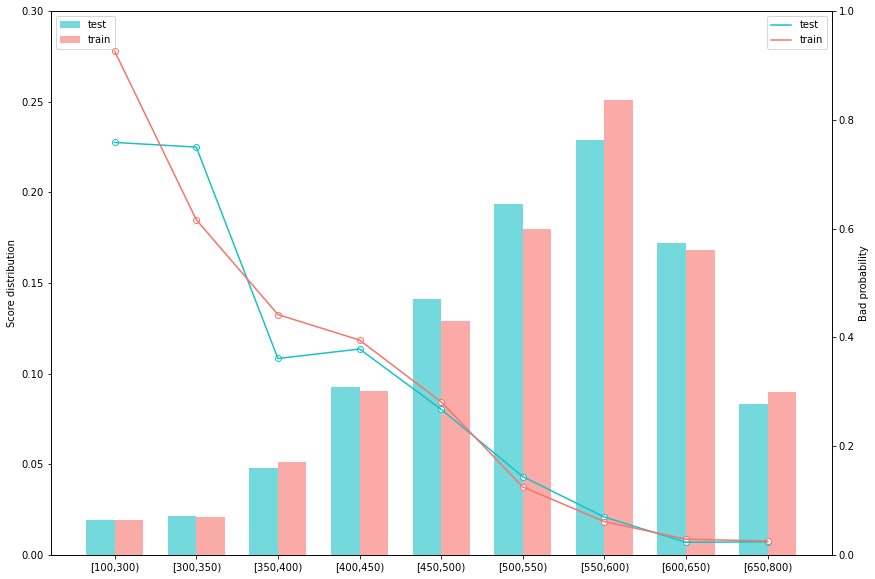
\includegraphics[scale=0.75]{figs/scorecard_plot.png}
	\caption{Scorecard Plot \label{scorecard_plot}}
\end{center}
\end{figure}
\end{landscape}

%\section{Ridge Regression}
%The Ridge Regression method or also know as Tikhonov regularization originally began being developed by Andre Tikhonov in Russia and published in the book "Solutions of ill-posed problems". During around the same time as Andre. two American statiticians, Arthur Hoerl and Robert Kennardcan, released the paper "Ridge Regression: Biased Estimation for Nonorthogonal Problems" in 1970. Ridge regression can be useful to apply when there is a large number of predictors which all seem to have a small effect on the response variable of interest. Applying ridge regression to the data produces a shrinking effect on the predictors and some can effectively reach zero but the method cannot reduce the estimates to exactly zero. As the coefficients shrink this does produce bias but also reduces the variance of the estimates.\cite{hoerl1970ridge}\cite{marquardt1975ridge}\\
%
%\paragraph{\textbf{Ridge Estimate}}Assume $\bm{X}$ is a $n$ by $p$ matrix and $\bm{Y}$ is an $n$ vector. The ridge regression estimator is given by:
%
%\begin{equation}
%\hat{\bm{\beta}}_{ridge} = (\bm{X^{'} X} + \lambda \bm{I}_p)^{-1} \bm{X^{'} Y}
%\end{equation}
%
%or can be seen as the values minimizing\cite{james2013introduction}:
%
%\begin{equation}
%\sum\limits_{i=1}^n\left(y_i-\beta_0-\sum\limits_{j=1}^p\beta_j x_{ij}\right)^2 + \lambda\sum\limits_{j=1}^p\beta_j^2=RSS + \lambda\sum\limits_{j=1}^p\beta_j^2
%\end{equation}
%
%Or similarly can be seen as:
%
%\begin{equation}
%\hat{\bm{\beta}} = arg \min\limits_{\bm{\beta}} \sum\limits_{i=1}^n \left(y_i-\sum\limits_{j=1}^p x_{ij}\beta_j \right)^2 \text{ subject to } \sum\limits_{j=1}^p \beta_j^2 < t
%\end{equation}
%
%where t is the tuning parameter.\\
%
%$\sum\limits_{j=1}^p \beta_j^2 < t$ is called the shrinkage penalty and can become very small when $\beta_1 ... \beta_p$ are close to zero. This shrinking penalty is not applied to our intercept as we only want to shrink the variables estimators. When our tuning parameter, $\lambda$, is set to zero, we are able to produce least squares estimates and for every possible value for $\lambda$ we will produce a different set of estimates for our predictors. Because of this it is important that the selection for the tuning parameter is as optimal as possible. Choosing the right value for the tuning parameter is also important to keep bias to a minimum while also reducing the variance of the estimates as much as possible.\cite{friedman2001elements} \\
%
%One way to select and appropriate value for $\lambda$ is through cross-validation. In order to do this we take a range of values for $\lambda$ and pick the value of $\lambda$ at which the cross-validation error is smallest.\\
%
%Although the ridge regression can be effective, the large problem if I was to use only this method would be that I am unable to reduce the amount of predictors used. Since the method is unable to exclude predictors and simply reduces redundant ones to very small values, the model will end up containing all 13 variables. There are many problems for this and sometimes is not ideal.\\
%
%\section{LASSO}
%LASSO(Least absolute shrinkage and selection operator) was first proposed by Robert Tibshirani\cite{tibshirani1996regression} in 1996. Introduced as an alternative for Ridge regression, The LASSO method is designed to minimize the residual sum of squares through an L1-norm. LASSO penalizes through an L1-norm (least absolute deviations) which minimizes the sum of the absolute differences. Sometimes this can result in reducing a coefficient to effectively zero. Providing what the method believes to be the most significant predictors. LASSO similar to ridge is a penalized regression method and produces bias in order to decrease the variance of the coefficients.
%\begin{defn}\cite{tibshirani1996regression}
%Suppose that we have data $(\bm{x}^i, y_i)$, $i=1,2,...,N$, where $\bm{x}^i = (x_{i1},...,x_{ip})^T$ are the predictor variables and $y_i$ are the responses. As in the usual regression set-up, we assume either that the observations and independent or that the $y_i$s are conditionally independent given the $x_{ij}$s. We assume that the $x_{ij}$ are standardized so that $\Sigma_i x_{ij}/N = 0$, $\Sigma_i x^2_{ij}/N = 1$.\\
%\\
%
%\paragraph{\textbf{LASSO Estimate}}
%The LASSO estimates can be found by minimizing this problem\cite{james2013introduction}:
%
%\begin{equation}
%\sum\limits_{i=1}^n\left(y_i-\beta_0-\sum\limits_{j=1}^p\beta_j x_{ij}\right)^2 + \lambda\sum\limits_{j=1}^p|\beta_j|=RSS + \lambda\sum\limits_{j=1}^p|\beta_j|
%\end{equation}
%
%Or similarly by letting $\bm{\hat{\beta}}=(\hat{\beta}_1,...,\hat{\beta}_p)^T$, the lasso estimate $(\hat{\alpha}, \hat{\beta})$ is defined by
%
%\begin{equation}
%(\hat{\alpha},\hat{\beta})=arg \min{\left\lbrace\sum\limits_{i=1}^N\left(y_i - \alpha - \sum\limits_j \beta_j x_{ij}\right)^2\right\rbrace} \qquad  \text{Subject to }\sum\limits_j |\beta_j| \leq t
%\end{equation}
%
%Where $t\geq0$ is a tuning parameter. $t$ controls the amount of shrinkage that is applied to the estimates.
%\end{defn}
%
%As you can see, Ridge and LASSO are fairly similar with the difference being in the shrinkage penalty. For Ridge we have $\beta_j^2$ and for LASSO we have $|\beta_j|$. Just like Ridge regression, LASSO has a shrinking effect on the predictors but with LASSO's shrinking penalty some estimates can be shrunk enough to be set to exactly zero effectively removing some variables. This produces a variable selection method, giving us a smaller model for interpretation. So as is with Ridge regression, it is important that we choose a suitable value for $\lambda$ and we can again use cross-validation to find that suitable value.\cite{friedman2001elements}
%
%\section{Elastic Net}
%The Elastic Net method is known to be a combination of both Ridge regression and Lasso, allowing the coefficients to be shrunk and in some cases set to zero. Introduced by Zou, Hui, and Trevor Hastie, It is considered, based on real world data and simulations, to out perform the LASSO method\cite{zou2005regularization}. One of the effects of the Elastic Net is that it causes grouping. Predictors which have strong correlations between each other are usually either left in or out together.\cite{zou2005regularization}\\
%\\
%In the paper by Hui and Hastie, they first define the Naive Elastic Net.
%\begin{defn}\cite{zou2005regularization}
%Suppose that the data set has $n$ observations with $p$ predictors. Let $\bm{y} = (y_1,..., y_n)^T$ be the response and $\bm{X} = (\bm{x}_1|...|\bm{x}_p)$ be the model matrix, where $\bm{x}_j = (x_{1j},..., x_{nj})^T, \quad j =1,...,p$, are the predictors. After a location and scale transformation, we can assume that the response is centred and the predictors are standardized,
%
%\begin{equation}
%\sum\limits_{i=1}^n y_i=0, \quad \sum\limits_{i=1}^n x_{ij}=0, \quad \text{and } \sum\limits_{i=1}^n x_{ij}^2=1, \qquad \text{for } j=1,2,...,p
%\end{equation}
%
%The naive elastic net estimate can be determined by minimizing
%
%\begin{equation}
%\hat{\bm{\beta}}= arg \min\limits_{\bm{\beta}} \left\lbrace \vert Y - \bm{X\beta} \vert^2 +\lambda_2\vert\bm{\beta}\vert^2 + \lambda_1\vert\bm{\beta}\vert_1 \right\rbrace
%\end{equation}
%
%where 
%
%\begin{equation}
%\vert\bm{\beta}\vert^2 = \sum\limits_{j=1}^p \beta_j^2 \text{ and } \vert\bm{\beta}\vert_1 = \sum\limits_{j=1}^p \vert\beta_j\vert 
%\end{equation}
%
%By letting $\alpha = \frac{\lambda_1}{\lambda_1 + \lambda_2}$, solving $\hat{\beta}$ can be seen as optimizing:\cite{Net}
%
%\begin{equation}
%\hat{\bm{\beta}} = arg \min\limits_{\bm{\beta}} \vert Y - \bm{X\beta} \vert^2, \text{ subject to } (1-\alpha)\vert\beta\vert_1 + \alpha\vert\beta\vert^2 \leq t \text{ for some t.}
%\end{equation}
%
%$(1-\alpha)\vert\beta\vert_1 + \alpha\vert\beta\vert^2$ is considered the elastic net penalty\cite{zou2005regularization}, which is a convex combination of the lasso and ridge penalty. Where letting $\alpha = 1$ causes a ridge penalty and $\alpha = 0$ allows a lasso penalty to be applied.
%\end{defn}
%
%Although the method still needs improvement. Using the naive elastic estimate brings a result similar to either a Ridge regression or a Lasso regression and does not produce a combination of both when applied. It produces an effect of shrinking the estimates twice as both the ridge and lasso methods produce shrinking. To solve this the elastic net estimate is provided. which is simply a rescaled estimate of the naive elastic estimate:
%
%\begin{equation}
%\hat{\bm{\beta}}\text{(elastic net)} = (1 + \lambda_2)\hat{\bm{\beta}}\text{(naive elastic net)}
%\end{equation}
%
%\section{Information Criterions}
%
%Once I have produced all three models from my methods I will need to select the one which fits my data the best. I have decided to use two information criterions, Akiake's\cite{hu2007akaike} and Bayesian's to select my final model.\\
%
%\begin{defn}\cite{posada2004model}
%The AIC for a given model is a function of its maximized likelihood (L) and the number of estimable parameters (K):
%
%\begin{equation}
%AIC = -2log(L) + 2K
%\end{equation}
%\end{defn}
%
%\begin{defn}\cite{posada2004model}
%The Bayesian Information Criterion (BIC) for a given model is:
%
%\begin{equation}
%BIC = -2log(L) + klog(n)
%\end{equation}
%
%where L is the maximized likelihood, k is the number of estimable parameters, and n is the given sample size.
%\end{defn}
%
%AIC and BIC are both a measure of goodness of fit by evaluating the loss of information from estimating the model. The smaller the values of these are the "better" the model is fitted. The reason I decided to use both is because of the different advantages and disadvantages each provide. AIC's main problem is the inability to compare models of different data sets, comparing the value of AIC's from a data set with $n=100$ and a data set with $n=80$ is meaningless. AIC tends to favour more complex models for large sample data's as an additional parameter has less of an impact, where as BIC penalises complex models more and tends to favour smaller models. 
%
%\section{In R}
%
%I will be using R studio to apply all of the methods to the data. The package which will be used in R studio is glmnet.\cite{hastie2014glmnet} This package is used to fit generalised linear models via penalised maximum likelihood by solving this problem:
%
%\begin{equation}
%\min\limits_{\beta_0,\beta}\frac{1}{N}\sum\limits_{i=1}^N w_i l \left( y_i,\beta_0 + \beta^T x_i \right) + \lambda\left[\left(1 - \alpha \right) ||\beta||_2^2/2 + \alpha ||\beta||_1 \right],
%\end{equation}
%
%where $l(y,\eta)$ is the negative log-likelihood contribution for observation i. By changing the value of $\alpha$ I can use this package for all three methods. With alpha at 0 it gives us ridge regression. With alpha at 1 allows us to solve by LASSO and in between provides elastic net. The package can be further read about in the publication "Regularization Paths for Generalized Linear Models via Coordinate Descent"\cite{friedman2010regularization} by Friedman, Jerome, Trevor Hastie and Rob Tibshirani where they explain further about the algorithms used in the package.\\
%
%The function I will be using is cv.glmnet(x, y, alpha = $\alpha$) which does a k-fold cross-validation for glmnet and returns a glmnet fit and a value for lambda. the inputs for alpha will be 0,1 and 0.5 for elastic net. Even though anywhere in between creates an elastic net method. I decided to go with 0.5 to make sure the ridge and lasso penalties are the same. 


\chapter{Modelling} \label{chapter:4}

\section{Logistic Regression Results}

For the modelling, the data was split into train and test sets with proportions 0.7 and 0.3 respectively. The bad rate was maintained in each data at 17\% to ensure fairness and the variables were converted to their woe values for their respective bin from tables  (\ref{woe_1}) \& (\ref{woe_2}). Once split, the train data was passed through a glm model with logit link, for this the python package statsmodels was used \parencite{statsmodels}. Three models were created, first, seen in Table (\ref{table:results_1}), was the base model with every variable included with no changes. Looking at the results table we can see that the majority of variables are highly significant with p-values less than 0.001. Mortdue is deemed the most insignificant, most likely due to its high correlation with VALUE and as such the variance it explains is already captured by VALUE. This is confirmed if we run the model again with VALUE dropped, seen in Table (\ref{table:results_val_dropped}). The p-value for MORTDUE is now 0.0005. \\

For the second model we looked at applying log transformations to the variables which had a heavy right skew, LOAN, MORTDUE, VALUE and YOJ to try to improve their p-values. These values were then passed through the woe binning and the values converted. The IV of LOAN and YOJ improved by 0.01 and 0.03 respectively whilst MORTDUE and VALUE's IV decreased, based on this, only the log transformations of LOAN and YOJ were kept and used for the second model. The results for the second model can be seen in Table (\ref{table:results_2}). \\

Finally, a third model was made from dropping variables with high p-values, these were MORTDUE and REASON. The results are displayed in Table (\ref{table:results_3}). All the remaining variables have a p-value of less than 0.0001. Every coefficient is positive, implying that an increase in all variables increase in the probability of BAD, which from initial observation shouldn't be right. Looking back on Section (\ref{sec:variables}) we have some assumptions of large values decreasing the probability of BAD such as CLAGE and YOJ. The reason for this is a result of the WOE methods, changing the values of our binned variables to their respective WOE value seen in Tables (\ref{woe_1}) \& (\ref{woe_2}). Higher values of CLAGE have negative values, for example values of CLAGE between 180 and 240 have a woe value of -0.47. So in reality, a CLAGE value in this range would have the effect of decreasing the probability of BAD. \\

\begin{table}[H]
\renewcommand{\arraystretch}{1.25}
\begin{center}
\begin{tabular}{llll}
\hline
Model:              & GLM              & AIC:            & 2514.3936    \\
Link Function:      & logit            & BIC:            & -25781.2585  \\
Dependent Variable: & BAD              & Log-Likelihood: & -1245.2      \\
\hline
\end{tabular}
\end{center}
\begin{center}
\begin{tabular}{lrrrrrr}
\hline
             &  Coef.  & Std.Err. &    z     & P$> |$z$|$ &  [0.025 &  0.975]  \\
\hline
\hline
const        & -1.5770 &   0.0539 & -29.2635 &      0.0000 & -1.6826 & -1.4714  \\
DELINQ\_woe  &  1.0403 &   0.0790 &  13.1746 &      0.0000 &  0.8855 &  1.1951  \\
CLAGE\_woe   &  0.9281 &   0.1005 &   9.2313 &      0.0000 &  0.7311 &  1.1252  \\
NINQ\_woe    &  1.0073 &   0.1533 &   6.5722 &      0.0000 &  0.7069 &  1.3077  \\
MORTDUE\_woe & -0.1110 &   0.2344 &  -0.4737 &      0.6357 & -0.5705 &  0.3484  \\
CLNO\_woe    &  0.8184 &   0.1343 &   6.0959 &      0.0000 &  0.5553 &  1.0816  \\
LOAN\_woe    &  0.8540 &   0.1018 &   8.3890 &      0.0000 &  0.6545 &  1.0535  \\
REASON\_woe  & -0.4899 &   0.3985 &  -1.2295 &      0.2189 & -1.2709 &  0.2910  \\
JOB\_woe     &  0.8730 &   0.1629 &   5.3592 &      0.0000 &  0.5537 &  1.1923  \\
VALUE\_woe   &  0.8503 &   0.1535 &   5.5400 &      0.0000 &  0.5495 &  1.1512  \\
DEROG\_woe   &  0.7714 &   0.1046 &   7.3725 &      0.0000 &  0.5663 &  0.9764  \\
YOJ\_woe     &  0.8313 &   0.1992 &   4.1740 &      0.0000 &  0.4410 &  1.2217  \\
\hline
\end{tabular}
\end{center}
\caption{Results: Model 1 \label{table:results_1}}
\end{table}

\begin{table}[H]
\renewcommand{\arraystretch}{1.25}
\begin{center}
\begin{tabular}{llll}
\hline
Model:              & GLM              & AIC:            & 2494.3355    \\
Link Function:      & logit            & BIC:            & -25813.6256  \\
Dependent Variable: & BAD              & Log-Likelihood: & -1237.2      \\
\hline
\end{tabular}
\end{center}
\begin{center}
\begin{tabular}{lrrrrrr}
\hline
            &  Coef.  & Std.Err. &    z     & P$> |$z$|$ &  [0.025 &  0.975]  \\
\hline
\hline
const       & -1.5749 &   0.0540 & -29.1591 &      0.0000 & -1.6808 & -1.4691  \\
DELINQ\_woe &  1.0369 &   0.0791 &  13.1031 &      0.0000 &  0.8818 &  1.1920  \\
CLAGE\_woe  &  0.9499 &   0.1007 &   9.4281 &      0.0000 &  0.7524 &  1.1473  \\
NINQ\_woe   &  1.0102 &   0.1525 &   6.6229 &      0.0000 &  0.7112 &  1.3091  \\
CLNO\_woe   &  0.7860 &   0.1331 &   5.9031 &      0.0000 &  0.5250 &  1.0469  \\
LOAN\_woe   &  0.8042 &   0.0934 &   8.6116 &      0.0000 &  0.6212 &  0.9872  \\
JOB\_woe    &  0.8508 &   0.1630 &   5.2195 &      0.0000 &  0.5313 &  1.1703  \\
VALUE\_woe  &  0.7937 &   0.1230 &   6.4517 &      0.0000 &  0.5526 &  1.0348  \\
DEROG\_woe  &  0.7840 &   0.1048 &   7.4802 &      0.0000 &  0.5785 &  0.9894  \\
YOJ\_woe    &  0.8988 &   0.1660 &   5.4148 &      0.0000 &  0.5735 &  1.2241  \\
\hline
\end{tabular}
\end{center}
\caption{Results: Model 3 \label{table:results_3}}
\end{table}

The performance of each model is shown and compared in Table (\ref{perf_eval}). It can be seen from this table that based on the performance evaulation mentioned in Section (\ref{sec:perf_eval}). Model 2 and 3 appear to out perform Model 1. But, when comparing the Model 2 to 3, the difference between performance indicators becomes smaller. Model 3 improves on every performance indicator but only by a small margin when compared to the change from Model 1 to Model 2. Based on Table (\ref{perf_eval}) either Model 2 or 3 would be an appropriate choice but we will go with Model 3. Even though the AIC of model 3 is smaller, this is still only a difference of 1.08. Where as the log-likelihood has a difference of 1.5 with model 2 performing better. This implies that Model 3 is only considered better when evaluting the AIC because of the removal of two variables and being a smaller model. Despite this, Model 3 still out performs Model 2 in the other 3, it has a higher K-S Statisitc, meaning it's best point of seperation is stronger than Model 2, a higher GINI coefficient implies it has a higher discriminatory power and the higher divergence value tells us that the scorecard has a stronger seperation of the distribution of goods and bads. \\

\begin{table}[H]
\begin{center}
\renewcommand{\arraystretch}{1.25}
\begin{tabular}{lcccc}
\toprule
Model & AIC & KS & GINI & Divergence \\
Model 1 (Default) & 2514.39 & 0.4581 & 0.5956 & 1.3802  \\
Model 2 (Log transformations) & 2495.42 & 0.4814 & 0.6078 & 1.4439  \\
Model 3 (REASON and MORTDUE dropped) & 2494.34 & 0.4822 & 0.6116 & 1.4568 \\
\bottomrule
\end{tabular}
\caption{Performance Evaluation Results On Test \label{perf_eval}}
\end{center}
\end{table}

\section{Scorecard Building}

With the model selected we then needed to turn the logistic regression results into a readable scorecard. To do this, we again used the scorcard package in python \parencite{statsmodels} and used the function \textit{scorecard(bins, model, xcolumns, point0, odds0, pdo)}. The function takes the woe bins in Tables (\ref{woe_1}) \& (\ref{woe_2}) and the logistic coefficients from Table (\ref{table:results_3}) and develops a points system for each variable and their bins. The function uses Equation (\ref{eq:scorecard}) to calculate each bin's point value.\\

\begin{equation}\label{eq:scorecard}
Score_{i,j} = -\dfrac{pdo}{\ln(2)} \cdot WOE_{j} \cdot \beta_{i}
\end{equation}

where i is the ith variable, j is the jth bin of the ith variable and pdo is the points to double odds which for this project is assigned to 50. \\

The full table of scores for each bin can be found in the Appendix in Table (\ref{table:scorecard_points}). The total score of an applicant would then be the sum of these points for the respective bin the applicant falls into for each variable. This is demonstrated by the example of two applicants in Table (\ref{table:app_example}). We can see applicant 1 an ideal candidate, is requesting a large loan against a large equity. Their job is within the office category which has the lowest bad rate and no dergoatory marks or delinquencies against them. The scorecard assigns a score of 872 for this applicant. Applicant 2 on the other hand does not appear from inital obsevation, appealing to a lender. A relatively low loan against an average equity results in a lower potential profit against a weaker collateral. The applicant is self employeed, one of the riskier job categories and they also have a delinquent credit line. The scorecard assigned a score of 610 to this applicant. \\ 

\begin{table}[H]
\begin{center}
\begin{tabular}{lrrrr}
\toprule
& \multicolumn{2}{c}{Applicant 1} & \multicolumn{2}{c}{Applicant 2} \\
Variable & Observation & Score & Observation & Score \\
\midrule
BASE & & 701 & & 701 \\ 
LOAN & 9.93 & 27.0 & 8.51 & -89.0 \\
VALUE & 220886 & 44.0 & 82575 & 17.0 \\
JOB & Office & 30.0 & Self & -24.0 \\
YOJ & 2.639 & -2.0 & 2.08 & 14.0 \\
DEROG & 0 & 11.0 & 0 & 11.0 \\
DELINQ & 0 & 27.0 & 1 & -58.0 \\
CLAGE & 213.91 & 32.0 & 335.03 & 64.0\\
NINQ & 1 & -1.0 & 3 & -29.0 \\
CLNO & 32 & 3.0 & 42 & 3.0 \\
\midrule
Score &  & 872 &  & 610
\end{tabular}
\end{center}
\caption{Scorecard Applicant Example \label{table:app_example}}
\end{table}

In Figure (\ref{scorecard_plot}) the score of every applicant in the train and test data is plotted. The figure displays the distribution and bad probability for each set. You can see the distributions appear to follow the same trend but on the lower end seem to vary slightly, this is most likely due to the smaller sample size of clients that have been scored in this range. Going back to our two applicants we can take a look at what area they fall in. Applicant 1 is placed in the highest band and has a bad probability of less than 0.01, there would be no reason this applicant would not be approved for the loan based on our scorecard. Applicant 2 is placed into one of the lower bands with a bad rate around 0.35, wether this applicant would be accepted or reject would depend on where a lender choses their cut-off score to be. It could be possible that this applicant would land in their soft-cut off area and reviewed and accepted but what we do know is that based off this scorecard, applicant 2's chance of acceptance is relatively low. \\

The PSI value of our scorecard is 1.1\% indicating the two samples don't have a shift in population. In Figures (\ref{fig:sc_dist_train}) \& (\ref{fig:sc_dist_test}) we can also see a clear seperation of goods and bads within our scorecard with bads clearly on the lower end of the scorecard and goods on the upper. 

%\begin{figure}[!ht]
%	\centering
%	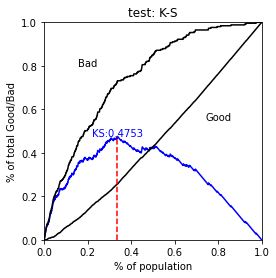
\includegraphics[scale=0.90]{figs/ks_plot.png}
%	\caption{KS Plot \label{ks_plot}}
%\end{figure}
%
%\begin{figure}[!ht]
%	\centering
%	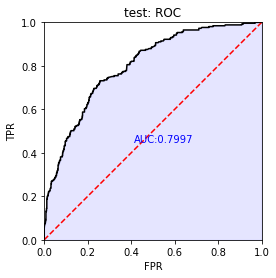
\includegraphics[scale=0.90]{figs/roc_plot.png}
%	\caption{ROC Plot \label{roc_plot}}
%\end{figure}

\begin{landscape}
\begin{figure}[!ht]
\begin{center}
	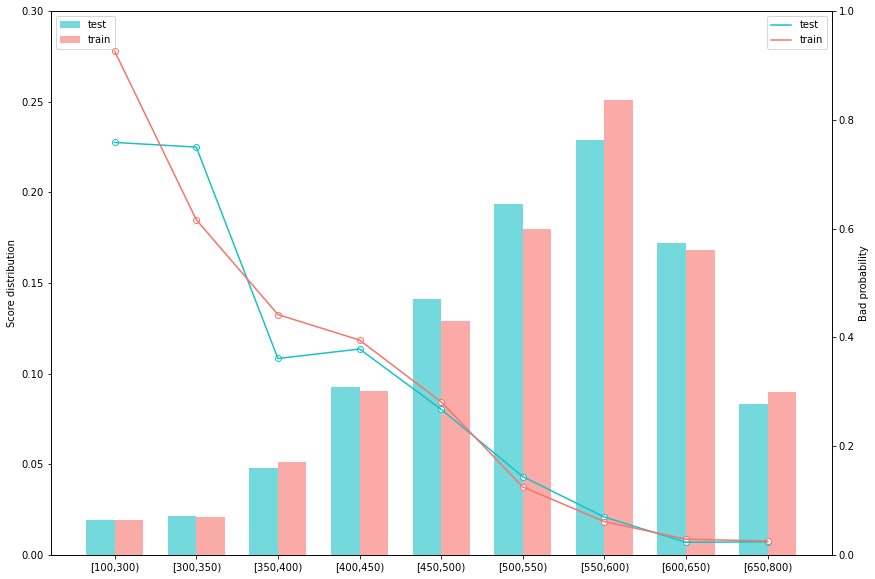
\includegraphics[scale=0.70]{figs/scorecard_plot.png}
	\caption{Scorecard Plot \label{scorecard_plot}}
\end{center}
\end{figure}
\end{landscape} 

\begin{figure}
\centering
  \centering
  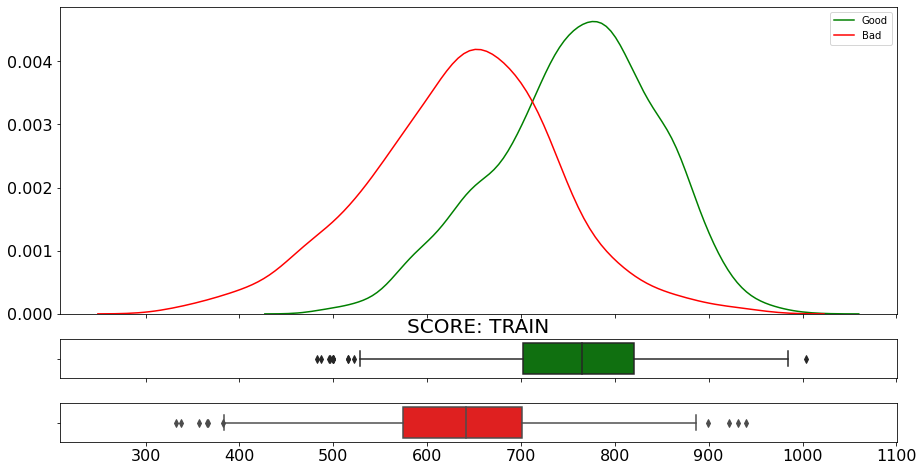
\includegraphics[width=0.9\linewidth]{figs/scorecard_dist_train.png}
  \caption{Scorecard Distribution for Train data}
  \label{fig:sc_dist_train}
\end{figure}

\begin{figure}
\centering
  \centering
  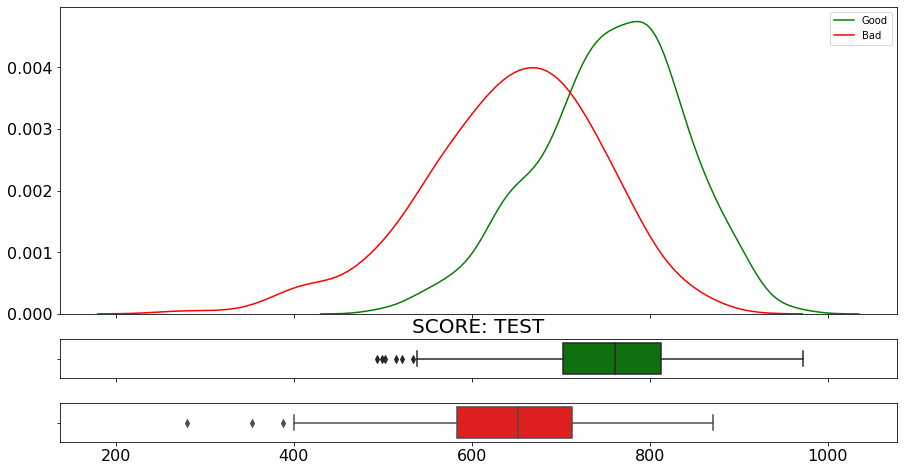
\includegraphics[width=0.9\linewidth]{figs/scorecard_dist_test.png}
  \caption{Scorecard Distribution for Test data}
  \label{fig:sc_dist_test}
\end{figure}


\chapter{Alternative Uses: Covid-19} \label{cha:chapter-4}
%
%I ended up producing 3 sets of Ridge, LASSO and Elastic Net models. The produced estimates for each model can be seen in  (\ref{Table4.1}), Table (\ref{Table4.2}) and Table (\ref{Table4.3}) along with their chosen $\lambda$ from cross validation and the RMSE for each model. I chose to use lambda.1se over lambda.min as the selected lambda since the documentation recommends this choice. The R code I used to produce the Ridge models is below, the code is the same for all three with alpha changed. Due to these being penalized regression methods, I needed to standardize my variables before I could use the function cv.glmnet. Because of the presence of the categorical variable CHAS, I needed to standardize the data without this variable. In order to do this I used the function scale() which produces the same effect of taking away the mean and dividing by the standard deviance for each observation.\\
%
%glmnet and cv.glmnet do not produce the standard errors for each estimation but there are methods to produce them but I decided against listing them with the coefficients. I did this because of the methods being penalizing. Due to the penalization creating high bias in the estimates, the standard errors nessacerily don't provide meaningful information for interpretation.\cite{goeman2016l1}.\\
%
%LASSO and Elastic Net have appeared to produce very similar results with removing the same variables and producing similar coefficients each time. This is most likely due to that Elastic Net is more suited to data with significantly more variables than observations allowing it to remove highly correlated variables together. In our results, when a variables was removed elastic net was seen more often removing two or more variables at the same time.\\
%
%When looking at our coefficient plots in figures (\ref{COEF1}), (\ref{COEF2}) and (\ref{COEF3}) we can look at how the methods shrink our coefficients and for LASSO and elastic net, which coefficients they drop off and when they do. I decided to plot the graphs of the full data to see the trend of all our variable's coefficients. From the graphs we can see that LSTAS was chosen to be kept in the longest for all three graphs and AGE was the first coefficient to be removed then after that, very quickly after that, ZN was removed. One interesting point is in the full data set with TAX still in, you can see TAX and RAD following an almost identical curve until RAD is just removed before TAX. After that the coefficient of TAX begins to increase in size again and ends up being removed after some other variables have been removed. This is almost certainly due to the high collinearity between them both along with the fairly similar correlation with the response variable. From this it is possible that removing RAD, even though it had the smaller inflation, would result in TAX being left in in the second model unlike RAD has been.\\
%
%\begin{lstlisting}[language=R]
%#Input Data
%Data <- read.table("boston.housing.data",header = T)
%x <- as.matrix(Data[,1:13])
%y <- as.matrix(Data[,14])
%#Remove CHAS and Standardize
%x.cont <- x[,-4]
%x.cont <- scale(x.cont)
%#Add CHAS
%x <- cbind(x.cont, x[,4])
%
%#Produce Glmnet Fit
%library(glmnet)
%set.seed(1) #Seed for reproduce ability
%cv.ridge <- cv.glmnet(x, log(y), alpha=0, standardize=FALSE)
%
%# Results
%plot(cv.ridge) #Plots mean square error
%plot(cv.ridge$glmnet.fit, xvar="lambda", label=TRUE) #Plots coef graphs
%cv.ridge$lambda.1se #Chosen lambda
%coef(cv.ridge, s=cv.ridge$lambda.1se) #Coefficient table
%cv.ridge$pred <- predict(cv.ridge, newx = x, s = "lambda.1se") #Predictions
%cv.ridge$rmse <- mean((log(y) - cv.ridge$pred)^2) #Root mean squared error
%cv.ridge$rmse 
%\end{lstlisting}
%
%\begin{figure}[ht]
%	\centering
%	\begin{tabular}{l r r r}
%	\multicolumn{4}{c}{Data Set 1}\\
%	Variable	&Ridge			&LASSO			&Elastic Net\\
%	\hline
%	$\lambda$ 	&0.110071		&0.007241934	&0.01448387\\
%	\hline
%	$\beta_0$	&3.032622800	&3.03403124		&3.034002936\\
%	CRIM     	&-0.064008179	&-0.06872488	&-0.067253625\\
%	ZN       	&0.009548101	&.         		&.          \\
%	INDUS    	&-0.013931833	&.         		&.          \\
%	NOX       	&-0.036593124	&-0.04825837	&-0.045162977\\
%	RM        	&0.086545058	&0.07600843		&0.078655535\\
%	AGE       	&-0.011898769	&.         		&.          \\
%	DIS       	&-0.047266508	&-0.05954217	&-0.054501993\\
%	RAD       	&0.017608700	&0.01960632		&0.014619337\\
%	TAX       	&-0.031845433	&-0.01698402	&-0.015810370\\
%	PTRATIO   	&-0.062793060	&-0.07399842	&-0.072136644\\
%	B         	&0.038056366	&0.03281628		&0.033099429\\
%	LSTAS     	&-0.143779730	&-0.20547168	&-0.199092357\\
%	CHAS      	&0.027325070	&0.00696304		&0.007372257\\
%	\hline
%	RMSE		&0.2013819		&0.1950815		&0.1959284\\	
%	\end{tabular}
%	\caption{Regression Estimates \label{Table4.1}}
%\end{figure}
%
%\begin{figure}[ht]
%	\centering
%	\begin{tabular}{l r r r}
%	\multicolumn{4}{c}{Data Set 2}\\
%	Variable	&Ridge 			&LASSO 			&Elastic Net\\
%	\hline
%	$\lambda$	&0.1208027		&0.01388938		&0.02531097\\
%	\hline
%	$\beta_0$ 	&3.0326787065	&3.03451287		&3.03451287\\
%	CRIM        &-0.0652516715	&-0.06246545	&-0.06313683\\
%	ZN          &0.0069716016	&.				&.\\
%	INDUS       &-0.0209047913	&.				&.\\
%	NOX         &-0.0387233569	&-0.02233285	&-0.02740610\\
%	RM          &0.0868841912	&0.07672957		&0.07999936\\
%	AGE         &-0.0128134450	&.				&.\\
%	DIS         &-0.0439698917	&-0.02848306	&-0.02898603\\
%	RAD         &0.0008558714	&.				&.\\
%	PTRATIO     &-0.0646415393	&-0.06629390	&-0.06694681\\
%	B           &0.0393031501	&0.02975365		&0.03133882\\
%	LSTAS       &-0.1413462017	&-0.20485916	&-0.19418048\\
%	CHAS        &0.0265168282	&.				&.\\
%	\hline
%	RMSE		&0.2036189		&0.2007459		&0.2007921\\
%	\end{tabular}
%	\caption{Regression Estimates after TAX is deleted \label{Table4.2}}
%\end{figure}
%
%\begin{figure}[ht]
%	\centering
%	\begin{tabular}{l r r r}
%	\multicolumn{4}{c}{Data Set 3}\\
%	Variable	&Ridge 			&LASSO 			&Elastic Net\\
%	\hline
%	$\lambda$	&0.1455073		&0.02923581		&0.05327716\\
%	\hline
%	$\beta_0$ 	&3.032739303	&3.03451287		&3.03451287\\
%	CRIM   		&-0.065804762	&-0.05420436	&-0.05721313\\
%	ZN      	&0.008897000	&.				&.\\
%	INDUS    	&-0.029853791	&.				&.\\
%	RM        	&0.088354647	&0.06957956		&0.07605300\\
%	AGE        	&-0.020492166	&.				&.\\
%	DIS    		&-0.035178628	&.				&.\\
%	RAD     	&-0.006112453	&.				&.\\
%	PTRATIO  	&-0.059708631	&-0.05531137	&-0.05661420\\
%	B         	&0.041403531	&0.02088837		&0.02590545\\
%	LSTAS      	&-0.144598353	&-0.20402847	&-0.18675554\\
%	CHAS        &0.025640770	&.				&.\\
%	\hline
%	RMSE		&0.2087332		&0.2087313		&0.2092953\\
%	\end{tabular}
%	\caption{Regression Estimates after TAX and NOX are deleted \label{Table4.3}}
%\end{figure}
%
%\begin{figure}[ht]
%	\centering
%	\includegraphics[scale=0.40]{figs/Plots1.pdf}
%	\caption{Mean Squared Error for Ridge \label{MSE1}}
%\end{figure}
%
%\begin{figure}[ht]
%	\centering
%	\includegraphics[scale=0.40]{figs/Plots2.pdf}
%	\caption{Mean Squared Error for LASSO \label{MSE2}}
%\end{figure}
%
%\begin{figure}[ht]
%	\centering
%	\includegraphics[scale=0.40]{figs/Plots3.pdf}
%	\caption{Mean Squared Error for Elastic Net \label{MSE3}}
%\end{figure}
%
%\begin{figure}[ht]
%	\centering
%	\includegraphics[scale=0.40]{figs/Plots4.pdf}
%	\caption{Mean Squared Error's Compared \label{MSE4}}
%\end{figure}
%
%\begin{landscape}
%\begin{figure}[ht]
%	\centering
%	\includegraphics[scale=0.65]{figs/PlotsC1.pdf}
%	\caption{Coefficient Plot for Ridge \label{COEF1}}
%\end{figure}
%\end{landscape}
%
%\begin{landscape}
%\begin{figure}[ht]
%	\centering
%	\includegraphics[scale=0.65]{figs/PlotsC2.pdf}
%	\caption{Coefficient Plot for LASSO \label{COEF2}}
%\end{figure}
%\end{landscape}
%
%\begin{landscape}
%\begin{figure}[ht]
%	\centering
%	\includegraphics[scale=0.65]{figs/PlotsC3.pdf}
%	\caption{Coefficient Plot for Elastic Net \label{COEF3}}
%\end{figure}
%\end{landscape}

\chapter{Conclusion} \label{cha:chapter-6}

Credit scores are something everyone will have an interaction with at some point in their lives and an important piece of personal finance. Scorecard modelling is a vital tool for financial insitutions to assist in evaluating their applicants. In this project we covered some of the popular methods used in credit scoring such as WOE and IV in Section (\ref{sec:woe_and_iv}) along with performance evaluation in Section (\ref{sec:perf_eval}). In Chapter 3 we explored a data set of home equity loans and the effect of some common variables have on the bad rate of applicants such as the number of times a client has been delinquent or the number of credit lines open. Using logisitc regression we were able to develop a selection scorecard for the dataset and evaluate the performance against each other. If we were to do anything different in this project, considering methods other than logistic regression such as support vector machines or decision trees would be our first choice, although logistic regression is the most popular for credit scoring due to its simplicity and reliabiltiy, there are these other methods which challenge its position. \\

We then demonstrated areas other than finance in which scorecard modelling and methods can be applied by using an open data set of covid-19 patients. Although the data set does not represet a true demographic for covid patients, it did allow us to see the potential use of scorecards to assess a patients risk. 

\begin{appendices}
\chapter{Definintions}

\textbf{Origination.} The period from when an client applies for a loan to its distribution of funds from the loan.\\

\textbf{Piggyback Lending.} An additional loan taken out on a property on top of the first mortgage.\\

\textbf{Subprime Loan.} A loan with higher interest rates, often given to clients with low credit score unable to qualify for normal rates. \\

\textbf{Goods.} The term to define a good client, most often meaning a client which does not default on a loan.\\

\textbf{Bads.} The term to define a bad client, most often meaning a client which ends up defaulting on a loan.\\

\textbf{Bad Rate.} The percentage of clients that have defaulted.\\

\chapter{Tables}

\begin{landscape}
\begin{figure}[ht]
	\centering
	\renewcommand{\arraystretch}{2}
	\begin{tabular}{lrrrrrrrrrrr}
	\toprule
	{} &     BAD &      LOAN &    MORTDUE &      VALUE &      YOJ &    DEROG &   DELINQ &    CLAGE &     NINQ &     CLNO &  DEBTINC \\
	\midrule
	count &  5621.0 &   5621.00 &    5278.00 &    5537.00 &  5294.00 &  5206.00 &  5356.00 &  5549.00 &  5422.00 &  5621.00 &  4447.00 \\
	mean  &     0.2 &  18846.02 &   73977.01 &  103025.40 &     9.00 &     0.24 &     0.45 &   179.77 &     1.19 &    21.45 &    34.07 \\
	std   &     0.4 &  11301.47 &   44813.54 &   58002.35 &     7.61 &     0.80 &     1.13 &    85.70 &     1.73 &    10.13 &     8.47 \\
	min   &     0.0 &   1100.00 &    2063.00 &    8000.00 &     0.00 &     0.00 &     0.00 &     0.00 &     0.00 &     0.00 &     0.52 \\
	25\%   &     0.0 &  11300.00 &   46385.00 &   66922.00 &     3.00 &     0.00 &     0.00 &   115.57 &     0.00 &    15.00 &    29.43 \\
	50\%   &     0.0 &  16500.00 &   65000.00 &   90008.00 &     7.00 &     0.00 &     0.00 &   173.63 &     1.00 &    20.00 &    35.02 \\
	75\%   &     0.0 &  23500.00 &   91989.25 &  120724.00 &    13.00 &     0.00 &     0.00 &   230.72 &     2.00 &    26.00 &    39.14 \\
	max   &     1.0 &  89900.00 &  399550.00 &  855909.00 &    41.00 &    10.00 &    15.00 &  1168.23 &    17.00 &    71.00 &   203.31 \\
	\bottomrule
	\end{tabular}
	\caption{Summary Before Outliers Removed \label{SUM_BFR_TBL}}
\end{figure}
\end{landscape}

\begin{landscape}
\begin{figure}[ht]
	\centering
	\renewcommand{\arraystretch}{2}
	\begin{tabular}{lrrrrrrrrrrr}
	\toprule
	{} &      BAD &      LOAN &    MORTDUE &      VALUE &      YOJ &    DEROG &   DELINQ &    CLAGE &     NINQ &     CLNO \\
	\midrule
	mean  &     0.18 &  17895.67 &   67997.48 &   97757.46 &     8.54 &     0.15 &     0.31 &   174.71 &     1.05 &    20.67 \\
	std   &     0.38 &   9543.89 &   36628.32 &   45795.23 &     6.89 &     0.48 &     0.76 &    75.72 &     1.34 &     9.00 \\
	min   &     0.00 &   1100.00 &    2063.00 &    8000.00 &     0.00 &     0.00 &     0.00 &     0.51 &     0.00 &     0.00 \\
	25\%   &     0.00 &  11000.00 &   43416.50 &   65783.00 &     3.00 &     0.00 &     0.00 &   115.08 &     0.00 &    14.00 \\
	50\%   &     0.00 &  16100.00 &   62344.00 &   88710.50 &     7.00 &     0.00 &     0.00 &   170.65 &     1.00 &    20.00 \\
	75\%   &     0.00 &  22800.00 &   86782.50 &  117303.00 &    12.00 &     0.00 &     0.00 &   224.57 &     2.00 &    26.00 \\
	max   &     1.00 &  60500.00 &  207687.00 &  270794.00 &    29.00 &     3.00 &     4.00 &   397.87 &     7.00 &    48.00 \\
	\bottomrule
	\end{tabular}
	\caption{Summary After Cleaning \label{SUM_AFT_TBL}}
\end{figure}
\end{landscape}

\begin{landscape}
\begin{figure}[ht]
	\centering
	\renewcommand{\arraystretch}{2}
	\begin{tabular}{lrrrrrrrrr}
		\toprule
		{} &   LOAN &  MORTDUE &   VALUE &     YOJ &   DEROG &  DELINQ &   CLAGE &    NINQ &    CLNO \\
		\midrule
		BAD       & -0.105 &  -0.0842 & -0.1049 & -0.0620 &  0.2175 &  0.2858 & -0.1820 &  0.1369 & -0.0632 \\
		LOAN       &     &   0.1730 &  0.3045 &  0.0453 &  0.0036 & -0.0946 &  0.1172 &  0.0661 &  0.1117 \\
		MORTDUE   &     &       &  0.8994 & -0.0693 & -0.0432 & -0.0424 &  0.1065 & -0.0061 &  0.3389 \\
		VALUE      &     &       &      & -0.0160 & -0.0570 & -0.0518 &  0.1775 & -0.0267 &  0.3107 \\
		YOJ        &     &       &      &      & -0.0464 &  0.0341 &  0.1669 & -0.0488 &  0.0307 \\
		DEROG      &     &       &      &      &      &  0.1680 & -0.0614 &  0.1249 &  0.0060 \\
		DELINQ     &     &       &      &      &      &      & -0.0108 &  0.0298 &  0.1101 \\
		CLAGE      &     &       &      &      &      &      &      & -0.0906 &  0.2202 \\
		NINQ       &     &       &      &      &      &      &      &      &  0.1046 \\
		\bottomrule
	\end{tabular}
	\caption{Correlation Table \label{CORR_TBL}}
\end{figure}
\end{landscape}

\begin{table}[H]
\renewcommand{\arraystretch}{1.25}
\begin{center}
\begin{tabular}{llll}
\hline
Model:              & GLM              & AIC:            & 2543.2467    \\
Link Function:      & logit            & BIC:            & -25758.5600  \\
Dependent Variable: & BAD              & Log-Likelihood: & -1260.6      \\
\hline
\end{tabular}
\end{center}
\begin{center}
\begin{tabular}{lrrrrrr}
\hline
             &  Coef.  & Std.Err. &    z     & P$> |$z$|$ &  [0.025 &  0.975]  \\
\hline
\hline
const        & -1.5661 &   0.0533 & -29.4073 &      0.0000 & -1.6705 & -1.4617  \\
CLNO\_woe    &  0.8257 &   0.1332 &   6.1991 &      0.0000 &  0.5646 &  1.0867  \\
YOJ\_woe     &  0.8134 &   0.1973 &   4.1221 &      0.0000 &  0.4267 &  1.2002  \\
REASON\_woe  & -0.4355 &   0.3941 &  -1.1049 &      0.2692 & -1.2080 &  0.3370  \\
LOAN\_woe    &  0.8959 &   0.1003 &   8.9325 &      0.0000 &  0.6994 &  1.0925  \\
JOB\_woe     &  0.8907 &   0.1612 &   5.5243 &      0.0000 &  0.5747 &  1.2067  \\
DELINQ\_woe  &  1.0305 &   0.0786 &  13.1048 &      0.0000 &  0.8764 &  1.1846  \\
DEROG\_woe   &  0.7534 &   0.1047 &   7.1983 &      0.0000 &  0.5482 &  0.9585  \\
MORTDUE\_woe &  0.6597 &   0.1889 &   3.4922 &      0.0005 &  0.2894 &  1.0299  \\
NINQ\_woe    &  1.0383 &   0.1520 &   6.8321 &      0.0000 &  0.7404 &  1.3362  \\
CLAGE\_woe   &  0.9666 &   0.1002 &   9.6503 &      0.0000 &  0.7703 &  1.1629  \\
\hline
\end{tabular}
\end{center}
\caption{Results: Model with VALUE dropped \label{table:results_val_dropped}}
\end{table}

\begin{table}[H]
\renewcommand{\arraystretch}{1.25}
\begin{center}
\begin{tabular}{llll}
\hline
Model:              & GLM              & AIC:            & 2495.4175    \\
Link Function:      & logit            & BIC:            & -25800.2346  \\
Dependent Variable: & BAD              & Log-Likelihood: & -1235.7      \\
\hline
\end{tabular}
\end{center}
\begin{center}
\begin{tabular}{lrrrrrr}
\hline
             &  Coef.  & Std.Err. &    z     & P$> |$z$|$ &  [0.025 &  0.975]  \\
\hline
\hline
const        & -1.5802 &   0.0542 & -29.1318 &      0.0000 & -1.6865 & -1.4738  \\
DELINQ\_woe  &  1.0393 &   0.0793 &  13.1121 &      0.0000 &  0.8839 &  1.1946  \\
CLAGE\_woe   &  0.9408 &   0.1010 &   9.3183 &      0.0000 &  0.7429 &  1.1387  \\
NINQ\_woe    &  0.9875 &   0.1533 &   6.4408 &      0.0000 &  0.6870 &  1.2880  \\
MORTDUE\_woe & -0.1417 &   0.2347 &  -0.6037 &      0.5461 & -0.6016 &  0.3183  \\
CLNO\_woe    &  0.8104 &   0.1347 &   6.0148 &      0.0000 &  0.5463 &  1.0744  \\
LOAN\_woe    &  0.8631 &   0.1002 &   8.6108 &      0.0000 &  0.6667 &  1.0596  \\
REASON\_woe  & -0.6331 &   0.4029 &  -1.5714 &      0.1161 & -1.4229 &  0.1566  \\
JOB\_woe     &  0.8575 &   0.1634 &   5.2485 &      0.0000 &  0.5373 &  1.1778  \\
VALUE\_woe   &  0.8590 &   0.1537 &   5.5879 &      0.0000 &  0.5577 &  1.1603  \\
DEROG\_woe   &  0.7875 &   0.1050 &   7.4994 &      0.0000 &  0.5817 &  0.9933  \\
YOJ\_woe     &  0.8890 &   0.1665 &   5.3401 &      0.0000 &  0.5627 &  1.2152  \\
\hline
\end{tabular}
\end{center}
\caption{Results: Model 2 \label{table:results_2}}
\end{table}


\chapter{Python Code}

\lstinputlisting[language=Python]{code/cleaning_script.py}

\lstinputlisting[language=Python]{code/exploratory_script.py}

\lstinputlisting[language=Python]{code/modelling_script.py}

\lstinputlisting[language=Python]{code/covid_19_script.py}

\end{appendices}


\printbibliography

\end{document}